\chapter{Diseño}
\label{cap:capitulo4}


\vspace{1cm}
El principal objetivo de este TFG es poder desarrollar un comportamiento de navegación autónoma en entornos de simulación 
con el fin de que el dron pueda alcanzar el comportamiento deseado utilizando inteligencia artificial, especificamente redes neuronales
y aprendizaje por refuerzo. Se tomará como entorno de simulación Airsim junto con el motor de videojuegos UnRealEngine, adicionalmente con 
la comunicación de este entorno con AirSim ROS Wrapper Node y Client Airsim a través de protocolos de red TCP/UDP, además del estudio y 
analisis de la comunicación entre Airsim, PX4 Autopilot, Mavros y AirSim ROS Wrapper Node .Así, pudiendo evaluar la unión de Airsim junto con ROS, PX4 y Mavros para
herramientas de diseño en la navegación autonóma de drones. \newline
\\

En primer lugar, en el contexto de la conducción autonóma de drones se evaluará el desarrollo de la percepción mediante redes neuronales y algoritmos de
aprendizaje no supervisado, en especial, clustering y regresiones. 
Posteriormente,el control del UAV se procederá una primera aproximación con un controlador Proporcional Derivativo Integral (PID) desenvolviéndose
en un entorno de carreteras de ambos carriles. \\
\\

Luego una vez de tener un comportamiento de sigue carril mediante el algoritmo de percepción desarrollado, procederemos a desarollar el algoritmo de 
aprendizaje por refuerzo. Junto con este aprendizaje se realizará analisis de diferentes métricas y resultados
por así entonces de poder encontrar una solución robusta y eficaz al problema que queremos enfrentarnos que será la navegación autonoma de drones en
entornos de carreteras.


\section{Diseño general}
\label{sec:Diseño general}
La primera aproximación que se llego a diseñar una infraestrutura para poder comunicar PX4 Autopilot y Mavros con Airsim. Para ello, tendremos
dos ordenadores en donde en el primer ordenador tendremos el simulador Airsim junto con UnRealEngine y en el segundo ordenador tendriamos 
PX4 Autopilot, ROS (con la distribución noetic), Mavros, Airsim ROS Wrapper y QGC. 


\begin{figure} [H]
    \begin{center}
      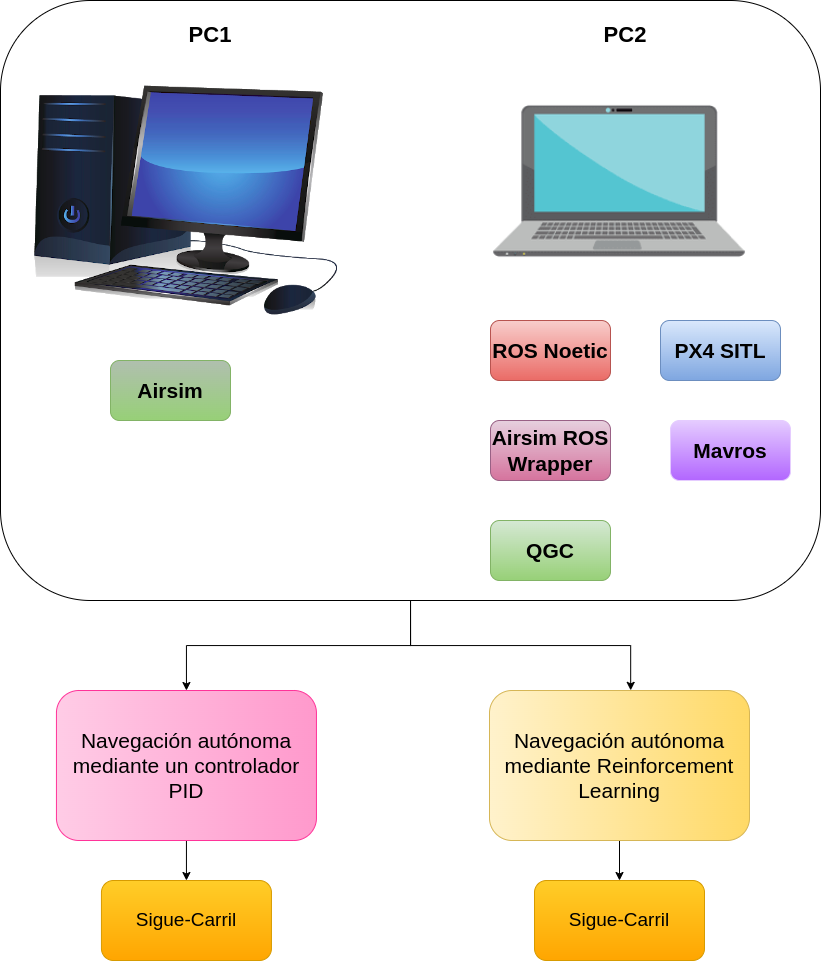
\includegraphics[scale=0.2]{figs/Diseño/Comunicaciones/digrama-general.drawio.png}
    \end{center}
    \caption{Primera aproximación de diseño de infraestructura}
    \label{fig:infraestructura}
  \end{figure}\

Por una parte tendremos dos ordenadores que se comunicaran entré si, el primer ordenador tendrá el simulador Airsim junto con el motor UnRealEngine y se comunicará a través
de protocolos TCP/UDP con el segundo ordenador. El segundo ordenador tendrá las plataformas de software, en las que daremos el comportamiento deseado al dron. 

A partir de ello, desarrollaremos la navegación autónoma realizando un comportamiento sigue carril mediante una red neuronal, clustering y algoritmos de aprendizaje supervisado. Este comportamiento
se llevará a dos enfoques: Desarrollar la navegación mediante un controlador proporcional derivativo integral y Reinforcement learning 

\section{Preparación del entorno}
\label{sec:Preparación_entorno}

Como mencionamos en la sección \ref{sec:simulación}, utilizaremos como simulador Airsim junto con el motor UnRealEngine. Para llevar acabo la construcción del entorno, primero tendremos 
que instalar UnrealEngine. Para ello, seguiremos las instrucciones marcadas por la página oficial de Epic Games \footnote{\textbf{Instalación}: \url{https://www.unrealengine.com/en-US/download}} y trabajaremos con la versión 4.27.2. 

Una vez se tenga UnRealEngine instalado, procederemos a configurar el entorno de simulación que necesitamos, para poder realizar este paso necesitaremos un fichero de configuración para definir el tipo de vehículo, sus sensores, la posición y las conexiones, dicho archivo se denomina settings.json

Un archivo settings.json es un archivo de configuración específica de Airsim que define cómo se ejecutará la simulación en términos de propiedades del vehículo, configuración de sensores, condiciones climatológicas y más. 

\subsection{Configuración del dron y del entorno}
\label{subsec:Configuración del dron y del entorno}

Como mencionamos, necesitamos un archivo de configuración para equipar al vehículo de sensores y otras características de comunicación con el entorno que son necesarias. 

Un archivo settings.json consta de varias secciones: 
\begin{enumerate}
  \item \textbf{SimMode}: Este parámetro define el modo de simulación, se refiere si el modo de simulación es para coches, multirotores o vision de computador. En nuestro caso
  utilizaremos multirotor. 
  \item \textbf{ClockType}: Determina qué tipo de reloj se utiliza para medir el tiempo en la simulación. En nuestro caso este parámetro estará vacío debido a 
  \item \textbf{Vehicles}:Configuración de  las propiedades de cada vehículo individualmente. Puedes especificar el tipo de vehículo, la posición inicial, la dinámica del vehículo, entre otros.
  En nuestro caso el tipo de vehículo que utilizaremos sera a partir de PX4 AutoPilot. Para utilizar este tipo de vehículo se debe configurar para ello las comunicaciones y 
  los diferentes parámetros de PX4 Autopilot. 
  \begin{itemize}
    \item \textbf{VehicleType}: En este caso ese parámetro tendremos un tipo de multirotor para PX4. Tomará el valor de PX4Multirotor
    \item \textbf{UseSerial}: Es para saber si vamos a usar un puerto serial en fisico, en nuestro caso como será simulado, por lo que dicho valor será False indicando que no 
    será utilizado.
    \item \textbf{LockStep}: Es una característica importante cuando se comunica con el simulador AirSim a través de TCP. Principalmente, sincroniza PX4 y el simulador para que utilicen esencialmente el mismo tiempo de reloj. 
    Esto permite que PX4 se comporte normalmente incluso durante demoras inusualmente largas en el rendimiento del simulador. Dicho valor valdrá True ya que lo utilizaremos. 
    \item \textbf{UseTcp}: Para poder comunicarnos a través de PX4 necesitamos habilitar esta opción a true.
    \item \textbf{TcpPort}: Especificamos el puerto TCP que vayamos a usar. 
    \item \textbf{ControlIp}: Esta opción se colocará con valor "remote" ya que el comportamiento será simulado y es remoto.
    \item \textbf{ControlPortLocal}: Se especificará el puerto Local del modo onboard de PX4 
    \item \textbf{ControlPortRemote}: Se especificará el puerto Remoto del modo onboard de PX4
    \item \textbf{LocalHostIp}: La dirección IP del ordenador en donde llevaremos la simulación, en este caso sera la dirección IP del primer ordenador.
    \item \textbf{Parameters}: Estos parametros son de PX4 y permite la configuración del vehiculo,
    como por ejemplo los modos de vuelo, sus configuraciones, configuraciones de velocidades y más. 
    \item \textbf{Sensors}:Permite personalizar la configuración de los sensores simulados, como Lidar, IMU (Unidad de Medición Inercial),GPS y sensor de distancia. 
    \item \textbf{Cameras}:Puedes configurar las cámaras utilizadas en la simulación, especificando sus propiedades como resolución, tipo de lente, posición y orientación relativas al vehículo.
    \newline 
    Nosotros usaremos una cámara que proporcionará una imagen RGB de dimensiones 620x620 pixeles y activaremos
    el flag de PublishToRos a 1 para poder acceder a ella mediante el Airsim ROS Wrapper con el topic /airsim\_node/PX4/front\_center\_custom/Scene. 
  \end{itemize}
\end{enumerate}
\begin{code}[H]
\begin{lstlisting}[language=json]
  {
   "SettingsVersion":1.2,
   "SimMode":"Multirotor",
   "ClockType":"SteppableClock",
   "ViewMode": "",
    "TimeOfDay": {
    "Enabled": true,
    "StartDateTime": "2023-08-12 22:00:00",
    "UpdateIntervalSecs": 1000000000,
    "CelestialClockSpeed":1
    },
   "Vehicles":{
      "PX4":{
         "VehicleType":"PX4Multirotor",
         "UseSerial":false,
         "LockStep":false,
         "UseTcp":true,
         "TcpPort":4560,
         "ControlIp":"remote",
         "ControlPortLocal":14540,
         "ControlPortRemote":14580,
         "LocalHostIp":"192.168.2.16",
         "Parameters":{
         "CBRK_IO_SAFETY":22027,
         "COM_ARM_CHK_ESCS":0,
         "COM_ARM_EKF_HGT":1.0,	
      	"COM_ARM_EKF_POS":1.0,	
         "COM_ARM_EKF_VEL":1.0,	
         "COM_ARM_EKF_YAW":1.0,	
	      "COM_FAIL_ACT_T":0.0,
         "COM_FLIGHT_UUID":0,
	      "COM_OBL_RC_ACT":5,
         "COM_PREARM_MODE":0,
         "FD_ACT_EN":0,
	      "LPE_LAT":47.641468,
         "LPE_LON":-122.140165,
	      "MIS_TAKEOFF_ALT":2.4,
         "MPC_TKO_SPEED":	5.0,
         "MPC_Z_VEL_MAX_DN":4.0,
         "MPC_Z_VEL_MAX_UP":8.0,
         "MPC_Z_V_AUTO_DN":4.0,
         "MPC_Z_V_AUTO_UP":8.0,
	      "NAV_DLL_ACT":0,
         "NAV_RCL_ACT":0,
	      "SIM_BAT_DRAIN": 86400,
	      "SIM_BAT_MIN_PCT": 100,
         "SYS_FAILURE_EN":0,
         "SYS_HITL":2
         },
        
\end{lstlisting}
\end{code}

\begin{code}[H]
  \begin{lstlisting}[language=json]
    "Sensors":{
            "Barometer":{
               "SensorType":1,
               "Enabled":true,
               "PressureFactorSigma":0.0001825
            },
            "Imu":{
               "SensorType":2,
               "Enabled":true
            },
            "LidarCustom":{
               "SensorType":6,
               "Enabled":true,
               "Range":10,
               "NumberOfChannels":16,
               "RotationsPerSecond":10,
               "PointsPerSecond":10000,
               "X":0,
               "Y":0,
               "Z":-1,
               "DrawDebugPoints":false,
               "DataFrame":"SensorLocalFrame"
            },
            "Gps":{
               "SensorType":3,
               "Enabled":true,
               "EphTimeConstant":0.9,
               "EpvTimeConstant":0.9,
               "EphInitial":25,
               "EpvInitial":25,
               "EphFinal":0.1,
               "EpvFinal":0.1,
               "EphMin3d":3,
               "EphMin2d":4,
               "UpdateLatency":0.2,
               "UpdateFrequency":50,
               "StartupDelay":1
            },
            "Distance":{
               "SensorType":5,
               "Enabled":true,
               "MinDistance":0.2,
               "MaxDistance":40,
               "X":0,
               "Y":0,
               "Z":-1,
               "Yaw":0,
               "Pitch":0,
               "Roll":0,
               "DrawDebugPoints":false
            }
        
        
  \end{lstlisting}
\end{code}

\begin{code}[H]
  \begin{lstlisting}[language=json]
    },
    "Cameras":{
            "front_center_custom":{
               "CaptureSettings":[
                  {
                     "PublishToRos":1,
                     "ImageType":0,
                     "Width":620,
                     "Height":620,
                     "FOV_Degrees":90,
                     "ImageRate_FPS":30,
                     "TargetGamma":1.5,
                     "AutoExposure":true,
                     "MotionBlur":false,
                     "PostProcess":true
                  }
               ],
               "X":0.50,
               "Y":0,
               "Z":0.10,
               "Pitch":0,
               "Roll":0,
               "Yaw":0
            }
         },
      "X": 22.474933624267578,
      "Y": -25.63629913330078,
      "Z":  0,
      "Pitch": 0,
      "Roll": 0,
      "Yaw":  30
      }
   }
}
  \end{lstlisting}
  \caption[Settings]{Archivo de configuracion settings.json}
  \label{cod:codejemplo}
\end{code}

  Dicho archivo se almacenará por defecto en Documentos en una carpeta creada por Airsim, si queremos cambiar dicha ruta o utilizar otro fichero de configuración distinto, solo bastará
  mencionar con el flag "\-settings" y la ruta absoluta de dicho archivo de configuraciones si queremos ejecutar el mapa de la simulación por linea de comando \newline
  
  Para poder ejecutar el simulador junto con la configuración realizada previamente, solo bastará ejecutar en una terminal de Windows (en nuestro caso será Windows, pero también
  se puede realizar en Linux, para ello vease https://microsoft.github.io/AirSim/settings/) ó en la propia carpeta del mundo ejecutable dadle doble click:


  IMAGENES DE LANZAMIENTO DEL SIMULADOR Y IMAGENES RESULTADOS DEL MUNDO

  \subsection{Configuración de los controladores}
  \label{subsec:Configuración controladores}

  Para poder comunicar Airsim ROS Wrapper,ROS no etic, PX4 , Mavros con el simulador, lo primero que realizaremos será la instalación de los cuatro componentes:
  \begin{enumerate}
    \item \textbf{PX4}: Para la instalación de PX4, procederemos a descargarnos el repositorio oficial en github con la version 1.14 \footnote{\textbf{Instalación PX4}: \url{https://github.com/PX4/PX4-Autopilot}}.
    Una vez se halla descargado, solamente se realizará la compilación a traves del comando: \texttt{make px4\_sitl\_default none\_iris} y tendremos que colocar como variable de entorno 
    \texttt{PX4\_SIM\_HOSTNAME} la dirección IP del primer ordenador, que es donde estará el simulador.

    Con ese comando, además de realizar la compilación y ejecutar PX4, también estamos especificando el tipo simulación y queremos que sea SITL y el tipo de vehículo .
    \item \textbf{Airsim ROS Wrapper}: Lo primero que se realizará sera la descarga del repositorio de Airsim a través de su pagina de github \footnote{\textbf{Instalación Airsim}: \url{https://github.com/microsoft/AirSim}}. 
    Cuando tengamos dicho repositorio descargado, lo que realizaremos sera la compilación y configuración de Airsim mediante los scripts build y setup
    \newline
    Ahora para poder utilizar el Airsim ROS Wrapper que nos proporciona ROS, tendremos que irnos a la carpeta dentro del repositorio de Airsim y buscar la carpeta de ros y construir el paquete 
    mediante el comando \texttt{catkin\_make}. Cuando tengamos realizado dicho paso tendremos que activar el wrapper en el fichero .bashrc de Linux mediante la siguiente linea:
    \texttt{source /home/\$USER/Airsim/ros/devel/setup.bashrc}
    \item \textbf{Mavros}: La instalación del paquete Mavros se puede seguir mediante el siguiente enlace \footnote{\textbf{Instalación Mavros}: \url{https://docs.px4.io/v1.14/en/ros/mavros_installation.html}}
    \item \textbf{ROS noetic}: Se seguirá la guía oficial de instalación de ROS \footnote{\textbf{Instalación ROS noetic}: \url{http://wiki.ros.org/noetic/Installation/Ubuntu}}

  \end{enumerate}

  Cuando se tenga todos los componentes instalados, se procederá a la comunicación de PX4,Mavros, Airsim ROS Wrapper. Una visión global de la insfraestructuras de comunicación se ilustra
  en la siguiente figura: 



  \begin{figure} [H]
    \begin{center}
      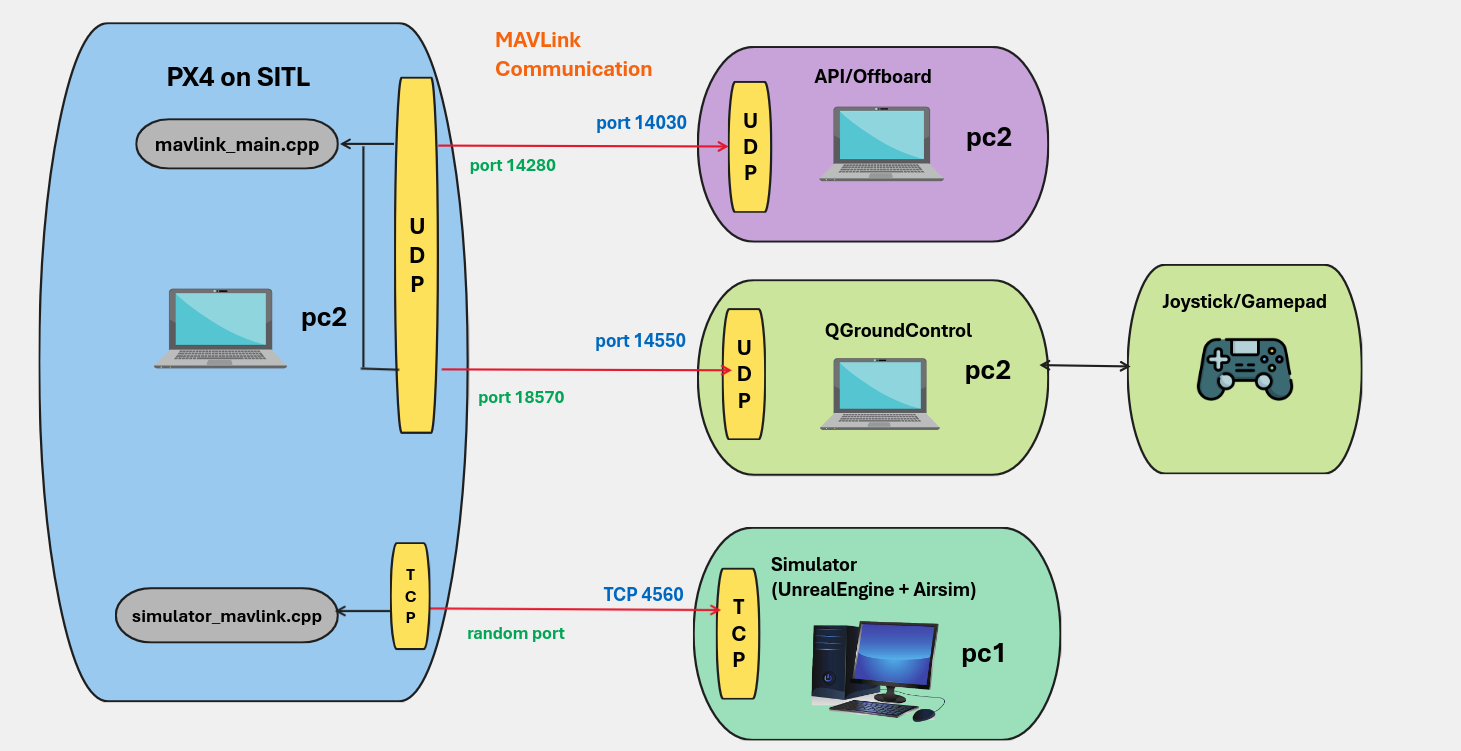
\includegraphics[width=0.9\textwidth,height=0.6\textwidth]{figs/Diseño/Comunicaciones/diagrama_comunicaciones.png}
    \end{center}
    \caption{Diagrama de comunicaciones entre PX4 y el simulador}
    \label{fig:ROS}
  \end{figure}\

  Como se puede observar, en el segundo ordenador tendremos PX4 STIL y se comunicará con el simulador a través de TCP con el puerto 4560, además se comunicará
  con la aplicación QGroundControl y la API de Mavros. Los puertos de comunicación que tiene PX4 SITL son escogidos por esta plataforma, dichos puertos se pueden observar
  cuando ejecutamos PX4 SITL

  \begin{figure} [H]
    \begin{center}
      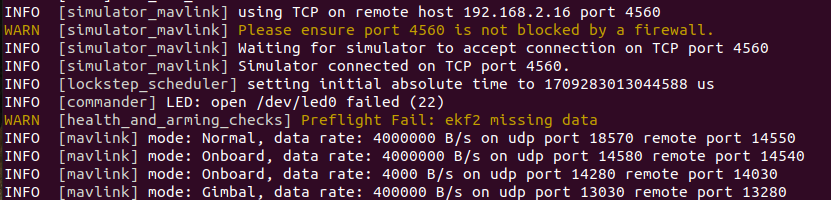
\includegraphics[width=0.7\textwidth,height=0.2\textwidth]{figs/Diseño/Comunicaciones/puertos.png}
    \end{center}
    \caption{Salida de la terminal ejecutando PX4 SITL}
    \label{fig:PX4_SITL}
  \end{figure}\

  

  
\newpage
\section{Percepción}
\label{sec:Percepción}
Para el desarrollo de la percepción una primera aproximación fue utilizar
procedimientos de visión clásica, es decir, procesar la imagen y mediante métodos de la libreria OpenCV \footnote{\textbf{OpenCV}: \url{https://opencv.org/}}
poder detectar las diferentes líneas que pueden haber en la carretera. El problema que nos podemos encontrar que al realizar esta primera proximación, al tener un 
entorno fotorrealista, estos métodos se quedan bastante pobres desembocando una percepción muy poco robusta e ineficiente. Por lo que se optó la utilización
de una red neuronal llamada YOLOP y algoritmos de aprendizaje automático poder construir la percepción. \newline

Para obtener la imagen del entorno nos la proporcionará AirSim ROS Wrapper Node, solamente nos subscribiremos al topic /airsim\_node/Drone/front\_center\_custom/Scene proporcionado por este
wrapper y utilizaremos un método de ROS denonimado CvBridge en donde podremos convertir dicha imagen en formato OpenCV y trabajar con ella a traves de OpenCv

\begin{figure} [H]
  \begin{center}
    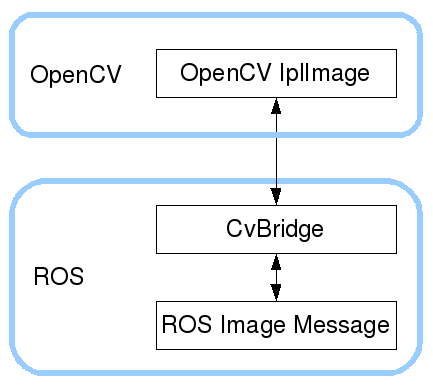
\includegraphics[width=0.6\textwidth,height=0.5\textwidth]{figs/Diseño/Percepcion/cvbridge.png}
  \end{center}
  \caption{Interfaz de Opencv con ROS utilizando CvBridge}
  \label{fig:CvBridge}
\end{figure}\

\newpage
\subsection{Inferencia de YOLOP}
\label{sec:Inferencia de YOLOP}

En este apartado hablaremos sobre la inferencia del YOLOP con sus distintos pesos preentrenados. En primer lugar, hablaremos
sobre los pesos End-to-end.pth y por último los pesos de Onnx.

Como anteriormente hemos comentado, el archivo End-to-end.pth es un archivo de pesos construido en Pytorch, cuando queremos cargar
dichos pesos con el modelo podemos hacerlo de dos maneras: Podemos realizarlo mediante la CPU o la GPU. 
Para ello, si queremos cargar el modelo de YOLOP con los pesos preentrenados End-to-end.pth se realizará de la siguiente forma:
\begin{code}[h]
  \begin{lstlisting}[language=Python]
  import torch
  
  model = torch.hub.load('hustvl/yolop', 'yolop', pretrained=True)

  \end{lstlisting}
  \caption[Cargar modelo YOLOP con pesos preentrenados End-to-end.pth]{Cargar modelo YOLOP con pesos preentrenados End-to-end.pth}
  \label{cod:codejemplo}
  \end{code}  

  Primero se cargará el modelo YOLOP a través de su repositorio de github \footnote{\url{https://github.com/hustvl/YOLOP}}
  , matizando el modelo de red neuronal y la opción "pretrained".A través de la última opción se escoge de su repositorio los pesos preentrenados con formato pytorch que
  en este caso es el archivo End-to-end.pth. Una vez tengamos el modelo cargado del repositorio, podemos escoger si queremos 
  hacer la inferencia en la CPU o GPU, para ello tendremos la siguiente linea de código: 

  
  \begin{code}[h]
    \begin{lstlisting}[language=Python]
   
    device = torch.device("cuda" if torch.cuda.is_available() else "cpu")
    model = model.to(device)
  
    \end{lstlisting}
    \caption[Cargar modelo YOLOP escogiendo como disposivo la GPU]{Cargar modelo YOLOP escogiendo como disposivo la GPU}
    \label{cod:codeloadYOLOP}
    \end{code}  

    En el \ref{cod:codeloadYOLOP} se puede observar que pytorch proporciona la opción de escoger entre CPU y GPU. En nuestro caso, escogeremos
    la GPU para realizar la inferencia y le asignaremos al modelo que realizaremos la inferencia por GPU. \newline

    Por último, nos quedaria convertir la imagen en un tensor antes de realizar la inferencia, una vez que se realice este paso
    se dará pie a la inferencia del modelo: 

    \begin{code}[h]
      \begin{lstlisting}[language=Python]
     
        from torchvision import transforms

        transform = transforms.ToTensor() 
                    
      imagen_tensor = transform(cv_image).to(device).unsqueeze(0)
      _, da_seg_out, ll_seg_out = self.model(imagen_tensor)
    
      \end{lstlisting}
      \caption[Inferencia del modelo]{Inferencia del modelo}
      \label{cod:codejemplo}
      \end{code}  

    Para poder convertir la imagen en un tensor, utilizaremos la funcion transforms.toTensor y después añadiremos una dimensión más con unsqueeze(0) , esto se debe 
    a que el modelo de YOLOP espera una entrada específica llamada batch\_size. Batch\_size es el número de imagenes que se procesarán juntas
    (generalmente 1 para inferencia) por lo que el tensor tendrá esta forma: (batch\_size, channels, height, width) \break. 

    Como resultado de la inferencia obtendremos un tensor de salida que corresponde la probabilidad de detencción de la Segmentación
    de la calzada y la detencciñon de las lineas de la calzada. Dicho tensor habrá que convertirlo en una imagen para poder visualizar
    dicho resultado en una imagen. 
    Por ello, convertiremos el tensor en un array numpy y realizaremos una transformacion para cambiar las dimensiones de (H,W,C) 
    a (C,H,W) esto se realiza ya que en Opencv representa imagenes en formato Numpy array y se transpone las dimensiones porque las
    imagenes de Opencv tiene la forma de (H, W, C)\footnote{\url{https://lindevs.com/convert-pytorch-tensor-to-opencv-image-using-python}}. Numpy es una libreria de Python por la cual podemos realizar operaciones de arrays
    \newline
    Una vez que hemos realizado esto, obtendremos un numpy array el cual lo normalizaremos con valores de 0-1, la tarea de normalizar 
    puede ayudar a igualar la escala de los pixeles de la imagen. Finalmente se podrá mostrar el resultado de la inferencia de la red 
    en una imagen, al normalizar los valores de 0-1, los valores que tengan un valor 1 se representarán en la imagen final y se le dará un color
    para que se pueda ver el resultado de la segmentación de la calzada y de la detencción de las lineas de la calzada.
    \newpage
    \begin{code}[h]
      \begin{lstlisting}[language=Python]
        import cv2
        import numpy as np
        for image in (da_seg_out,ll_seg_out):

          image_np = image.detach().cpu().numpy()
          image_array = np.transpose(image_np, (2, 3, 1, 0))

        
          image_norm = cv2.normalize(image_array[:,:,1,:], None, 0,1, cv2.NORM_MINMAX, cv2.CV_8U)

          images.append(image_norm)

    
        cv_image[images[0] == 1] = [0, 255, 0]
        cv_image[images[1] == 1] = [0, 0, 255]

        cv2.imshow('Image', cv_image)
        cv2.waitKey(1)

    
      \end{lstlisting}
      \caption[Resultado de la inferencia del modelo YOLOP]{Resultado de la inferencia del modelo YOLOP}
      \label{cod:codejemplo}
      \end{code}  

      Los pesos preentrenados de Onnx para poder utilizarlos en la inferencia del modelo YOLOP tendremos que descargarnos la libreria Onnx para Python, 
      seguiremos los pasos de la página oficial \footnote{\url{https://onnxruntime.ai/docs/install/}}
      Para saber que tipo de versión necesitamos instalar de OnnxRuntime para realizar la inferencia a traves de la GPU, tenemos que saber que versión de cuda
      tenemos, esto se puede saber ejecutando en una terminal el siguiente comando:  \texttt{nvidia-smi}. Con este comando nos saldrá este panel de información:

      \begin{figure} [H]
        \begin{center}
          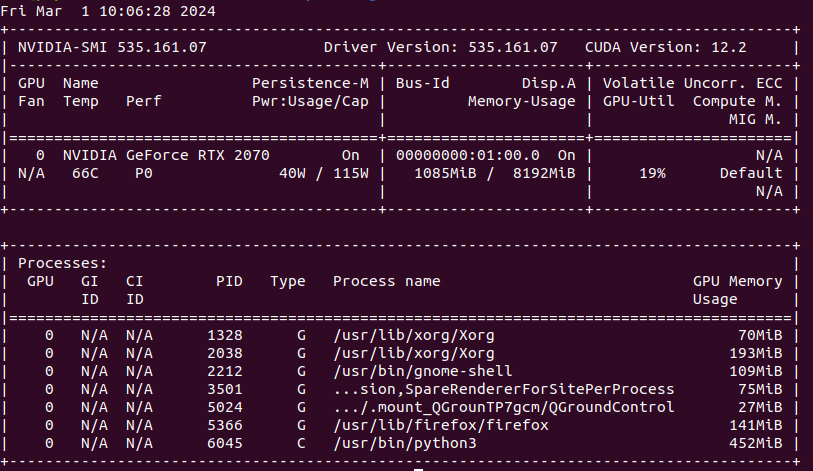
\includegraphics[width=0.6\textwidth,height=0.4\textwidth]{figs/Diseño/Percepcion/Panel-nvidia.png}
        \end{center}
        \caption{Panel de Nvidia}
        \label{fig:Nvidia}
      \end{figure}\

      En la esquina superior derecha, podemos ver que tenemos la version de CUDA de nuestro ordenador, en este caso tenemos la versión de CUDA 12.2 por lo que necesitamos una versión compatible
      para dicha versión. Para saber lo anterior, solamente bastará encontrar en la siguiente tabla de la página oficial de Onnx \footnote{\url{https://onnxruntime.ai/docs/execution-providers/CUDA-ExecutionProvider.html}} la versión compatible con nuestra versión de CUDA. \newline
      Cuando empezamos a realizar dicha instalación en diciembre de 2023, la versión que existia de onnx runtime solamente era compatible con CUDA 11.8, por lo tanto tuvimos que descargarnos 
      dicha versión de CUDA y colocar dicha variable de entorno la ruta en donde se encontraba la instalación de CUDA 11.8 \texttt{LD\_LIBRARY\_PATH=/usr/local/cuda-11.8/lib64:\$LD\_LIBRARY\_PATH} \break. 

      Cuando tengamos todo preparado y configurado ya podremos realizar los pasos de la inferencia con los pesos preentrenados de Onnx. En primer lugar,cargaremos el modelo
      
      \begin{code}[h]
        \begin{lstlisting}[language=Python]
          import onnxruntime as ort

          ROUTE_MODEL = "/home/bb6/YOLOP/weights/yolop-320-320.onnx"
          ort_session = ort.InferenceSession(ROUTE_MODEL,providers=['CUDAExecutionProvider'])
      
        \end{lstlisting}
        \caption[Cargar modelo]{Cargar modelo YOLOP-320-320.onnx}
        \label{cod:codejemplo}
        \end{code}  

        Como se observa en el código 4.5, a la hora de cargar el modelo escogemos como provider CUDAExecutionProvider. Cuando trabajamos con ONNX Runtime, 
        podemos especificar qué proveedores de ejecución utilizar para ejecutar el modelo ONNX que escojamos, cada proveedor contiene un conjunto de núcleos optimizados para un objetivo específico (por ejemplo, CPU, GPU, IoT) y 
        se especifican como una lista en el orden de prioridad. En nuestro caso escogeremos CUDA para ejecutar mediante la GPU. 
        \newline
        A continuación preprocesaremos las imagenes de entrada que le daremos al modelo, al escoger el modelo de yolop-320-320.onnx, las imagenes deben tener una dimensión de 320x320, para ello
        utilizaremos un método implementado por ellos, en el cuál redimensionaremos la imagen como se pide para el modelo. 
        Una vez que tengamos la imagen preparada, daremos comienzo a la inferencia del modelo de yolop-320-320.onnx. 
        \newpage

        \begin{code}[h]
          \begin{lstlisting}[language=Python]
            _, da_seg_out, ll_seg_out = self.ort_session.run(
              ['det_out', 'drive_area_seg', 'lane_line_seg'],
              input_feed={"images": img}
          )
        
          \end{lstlisting}
          \caption[Inferencia del modelo yolop-320-320.onnx]{Inferencia del modelo yolop-320-320.onnx}
          \label{cod:codejemplo}
          \end{code}  

        La inferencia del resto de modelos de Onnx se realizan de la misma forma pero teniendo en cuenta que se tendrá que cambiar las dimensiones de las imagenes de entrada y la ruta
        en donde se almacena dicho modelo. 


\subsubsection{Resultados de YOLOP }
\label{sec:resultados}
Anteriormente, estuvimos hablando sobre lo que ofrece YOLOP, su modelo en concreto y sus pesos preentrenados. En esta sección contrastaremos los resultados de cada parte mencionada. \newline
En la siguiente figura mostramos la media en realizar la inferencia de YOLOP utilizando los pesos preentrenados End-to-end.pth, yolop-320-320.onnx y yolop-640-640.onnx en segundos.

\begin{figure} [H]
  \begin{center}
    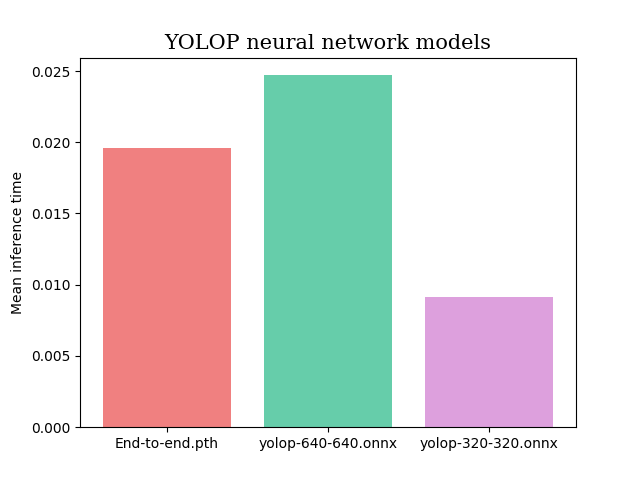
\includegraphics[scale=0.4]{figs/Diseño/Percepcion/Results-Yolop.png}
  \end{center}
  \caption{Resultados de los pesos preentrenados del modelo YOLOP}
  \label{fig:pesos_preentrenados}
\end{figure}\

Como podemos observar en la figura 4.6, los pesos preentrenados que tiene una inferencia menor al resto se trata de yolop-320-320.onnx, tiene un tiempo de inferencia alrededor de 0.010s, esto
significa que el modelo YOLOP con estos pesos tiene aproximadamente un rate de 100 FPS. Si comparamos este resultado con los restantes pesos, es el ganador en cuanto 
en tiempo de inferencia y rate. 
Onnx está diseñado para ser más eficiente en términos de memoria y velocidad de inferencia en cuanto Pytorch, lo que puede mejorar la velocidad y la precisión
del modelo, por lo que puede que el modelo tarde menos en inferir pero depende de varios factores. 

FOTOS DE LOS RESULTADOS DE LA RED



Una vez escogido el modelo yolop320-320.onnx procederemos a seleccionar las lineas detectadas que nos interesan.

\subsection{DBSCAN}
\label{sec:DBSCAN}

Para saber con qué lineas detectadas por la red nos quedaremos, utilizaremos un algoritmo de aprendizaje no supervisado llamado clustering, en particular
utilizaremos DBSCAN(Density-Based Spatial Clustering of Applications with Noise)\footnote{\url{https://scikit-learn.org/stable/modules/generated/sklearn.cluster.DBSCAN.html}}. 

DBSCAN es un algoritmo de agrupamiento no paramétrico que se encuentra en la librería scikit-learn. Scikit-learn\footnote{\url{https://scikit-learn.org/stable/}} es una libreria de Python para algoritmos de aprendizaje automático,
este algoritmo trabaja con muestras centrales de alta densidad y expande clústeres a partir de ellas. Es especialmente útil para datos que contienen clústeres de densidad similar.
\newline
Dicho algoritmo contiene varios parámetros que son importantes conocerlos y configurarlos: 
\begin{enumerate}
  \item \textbf{Eps}: Consiste en la distancia máxima que puede existir entre dos muestras para que una se considere vecina de la otra. Dicha distancia no se trata de un límite 
  máximo entre las distancias que puede haber dentro de un cluster.
  \item \textbf{Min\_samples}: Es el número mínimo de muestras dentro de un vecindario para que un punto se considere como un punto central incluyendo al propio punto.
  \item \textbf{Metric}: La métrica utilizada para calcular la distancia entre los conjuntos de clusteres (por defecto es la distancia euclidiana). 
\end{enumerate}
Los valores de los parámetros de la distancia máxima y el número mínimo de muestras se deben elegir cuidadosamente, es decir, si colocamos una distancia 
máxima alta puede provocar que los clusters que queramos que pertenezcan a un distinto grupo pertenezcan al mismo grupo. 
Si min\_samples se establece en un valor alto, DBSCAN encontrará clústeres más densos y 
si se establece en un valor bajo, los clústeres encontrados serán más dispersos.
\break
Por lo que para encontrar los valores de estos 2 parámetros fue experimentando y quedandonos con el mejor resultado. En nuestro caso la distancia máxima tendra un valor de 10 
y el número mínimo de muestras sera de 5 muestras. Lo que significa que la distancia máxima que tendrán los puntos para pertenecer al mismo grupo de clusteres sera de 10 de distancia en pixeles
con un mínimo de muestras pertenecientes de 5 muestras. 

Para entender un poco más como funciona el algoritmo, en la siguiente figura recogida por Research: 

\begin{figure} [H]
  \begin{center}
    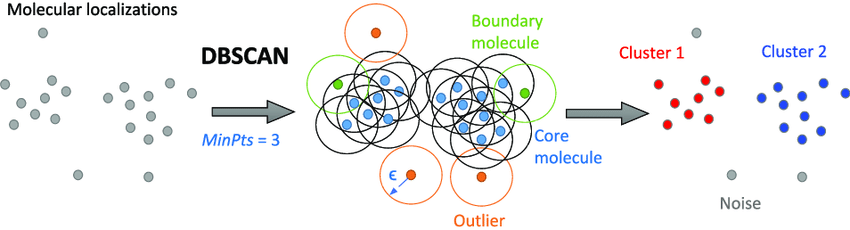
\includegraphics[width=0.8\textwidth,height=0.3\textwidth]{figs/Diseño/DBSCAN/DBSCAN-Illustration.png}
  \end{center}
  \caption{Resultados de los pesos preentrenados del modelo YOLOP}
  \label{fig:pesos_preentrenados}
\end{figure}\

En la figura \ref{fig:pesos_preentrenados} se ilustra un ejemplo teniendo un número de muestras ubicadas aproximadamente cercanas unas de otras. Aplicamos el algoritmo de DBSCAN 
teniendo como valor el número mínimo de muestras 3, eso significa que para que se considere una muestra a un grupo de cluster tendrá que tener una densidad de 3. El algoritmo itera por
las muestras y compara el valor de la distancia máxima y el número mínimo de muestras. 
Si ningún de estos dos parámetros no se cumpliese ya que puede darse que una muestra se encuentra lejana del grupo de muestras será etiquetado como ruido, esto quiere decir
que no pertenecerá a ningún grupo de clusteres. Dicho resultado se puede observar en la figura \ref{fig:pesos_preentrenados} como el algoritmo ha catalogado dos grupos de clusteres y 3 muestras
como puntos de ruido. 
\break

Centrandonos en nuestra implementación con el algoritmo de DBSCAN, le pasaremos la imagen de salida de la red neuronal pero con la particularidad que DBSCAN necesitaria que la imagen sea
representada por un array bidimensional de coordenadas x e y de puntos. Para ello utilizaremos la función de Numpy column\_stack, dicha función transforma un array simple de una dimensión a
un array de 2 dimensiones, una vez se realice esto obtendremos un array bidimensional para el algoritmo DBSCAN.\newline

Obtenemos el resultado de DBSCAN con los parámetros configurados de eps = 10 y min\_samples = 5, dicho resultado será una lista con etiquetas de 0 a n, siendo 0 el primer grupo de clusters detectado y 
n el último grupo de clusters detectado. De las listas de etiquetas se eliminarán los clusters que hallan sido etiquetados como ruido, para ello solo basta encontrar la etiqueta con valor -1 ya que
DBSCAN cataloga las muestras ruidosas con -1 y para obtener el resultado solamente bastará iterar en dicha lista y mostrar los puntos correspondientes de cada etiqueta en la imagen de salida


Una vez realizado el algoritmo de DBSCAN necesitamos quedarnos con el grupo de clusters que pertenezcan al carril que queremos seguir, para ello calcularemos los centroides de cada
grupo de clusters detectado y los clasificaremos en función de si se encuentran en la derecha o izquierda de la imagen, es decir, la imagen tiene unas dimensiones de 320x320 por lo tanto 
nos fijaremos en el valor del eje x en el ecuador con valor 160, por lo que cuando calculemos los clusters serán clasificados en función de los valores de x si se encuentran a la derecha u izquierda de 160 
que es la mitad de la imagen. 

Al clasificar de esta forma el grupo de clusters será más sencillo escoger cuales de la derecha e izquierda necesitamos, para ello escogeremos dichos grupos mediante una función máximizada
la cual escoge dicho grupo de clusters de la derecha u izquierda en función de la cercania de un punto central P escogido como valor (220,160) siendo 220 el valor de las y e 160 el valor de las x, 
es importante mencionar que cuando trabajamos con puntos en numpy las coordenadas estan dados la vuelta, es decir, en vez de estar (x,y) como estamos acostumbrados a trabajar están colocados
como (y,x). A parte de escoger en función de la cercania de un punto P también esta en función de la densidad de puntos de dicho grupo de clusters de la derecha u izquierda detectados, con
esto conseguimos que no solamente escojamos en función de la cercania si no que también lo haremos según la cantidad de puntos. \newline

\begin{code}[h]
  \begin{lstlisting}[language=Python]
    def score_cluster(self,cluster, center):
      points_cluster, centroid = cluster
    
      proximity = np.linalg.norm(centroid - center)
      density = len(points_cluster)
      return density / proximity

  \end{lstlisting}
  \caption[Función maximizada para escoger el grupo de cluster más cercano y denso respecto al punto P]{Función maximizada para escoger el grupo de cluster más cercano y denso respecto al punto P}
  \label{cod:codejemplo}
  \end{code}  

\begin{figure} [H]
  \begin{center}
    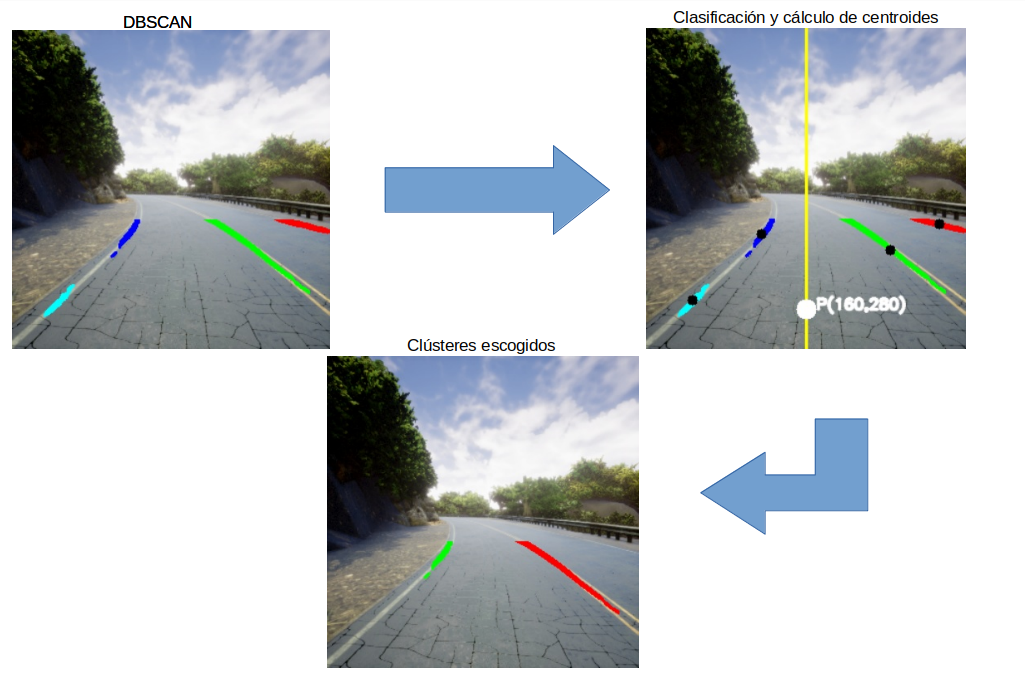
\includegraphics[scale=0.4]{figs/Diseño/DBSCAN/resultado.png}
  \end{center}
  \caption{Ilustración del proceso de elección de clústeres }
  \label{fig:DBSCAN_imagen}
\end{figure}\
Cuando tengamos el resultado de los clusters de la derecha e izquierda escogidos procederemos a realizar dos regresiones cuadráticas para construir las lineas del carril que queremos seguir.
\subsection{Regresión cuadrática}
\label{sec:Regresión cuadrática}
Como anteriormente hemos mencionado, cuando tengamos los clusters escogidos correctamente daremos pie a la construcción de dos regresiones cuadráticas. \newline 
\newline 
La regresión es un método de aprendizaje supervisado el cual consiste en aproximar un número N de puntos a una recta, curva, etc, en nuestro caso hemos escogido realizar una regresión cuadrática ya que el recorrido
que vamos a realizar las lineas detectadas por la red neuronal no son totalmente rectas si no que se tratan de lineas curvilineas por lo que la regresión cuadrática en este papel puede 
funcionar perfectamente. \newline

Para la construcción de las regresiones cuadráticas utilizaremos las funciones de la libreria Numpy denominada Polyfit\footnote{\url{https://numpy.org/doc/stable/reference/generated/numpy.polyfit.html}}
y Polyval\footnote{\url{ https://numpy.org/doc/stable/reference/generated/numpy.polyval.html}}. 
Polyfit es una función que calcula los  coeficientes del polinomio que mejor se ajusta a los datos utilizando el método de los mínimos 
cuadrados para la ecuación cuadrática,obtendremos tres coeficientes, denominados a,b y c. \newline
\newline
Con dichos coeficientes realizaremos una media de los últimos diez valores y por cada cinco iteraciones dicha media se volverá a calcular, este paso lo realizamos ya que 
queremos disminuir las oscilaciones causadas de las detencciones de la red neuronal. Una vez calculados los coeficientes, realizaremos la regresión cuadrática mediante la función Polyval, dicha función calcula
la función cuadrática con los coeficientes calculados anteriormente. \newline 
Una vez obtengamos los valores de la función cuadrática, realizaremos una clasificación para quedarnos con los puntos obtenidos
de dicha función los que se encuentren en el eje y entre los valores 0 a 319, esto se debe hacer ya que dicha función como resultado puede dar numeros negativos realizando dicha regresión y en una 
imagen no se trabaja con números negativos, lo cual habrá que seleccionar los puntos correspondientes donde se encuentran en la imagen para poder seleccionarlos \newline

Este proceso se realizará dos veces, una regresión cuadrática para el grupo de clusteres detectados escogidos de la derecha y otra regresión cuadrática para el grupo de clusteres detectados
escogidos de la izquierda. \newline
Finalmente, con dichas regresiones cuadráticas se realizará una dilatación de los puntos para tener un resultado más llamativo y visual al poder
ver las regresiones cuadráticas.\newline

\begin{figure} [H]
  \begin{center}
    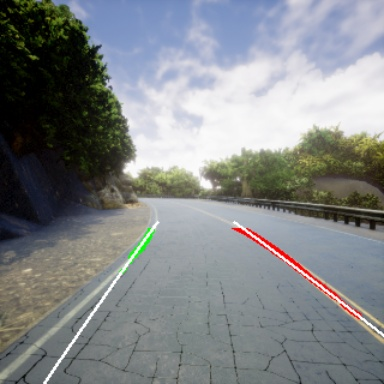
\includegraphics[scale=0.4]{figs/Diseño/Regresiones/regresion.jpg}
  \end{center}
  \caption{Resultado de la regresión cuadrática}
  \label{fig:regresión cuadrática}
\end{figure}\

\subsection{Interpolación y cálculo del centro de masas del carril}
\label{sec:Interpolación y cálculo del centro de masas del carril}

Una vez obtenido las lineas que nos interesa, necesitamos quedarnos con el carril que se encuentren contenido entre ambas lineas. Para ello realizaremos una interpolación que consiste en recorrer
los puntos de la imagen original y quedarnos con los puntos que se encuentren dentro de los límites de ambas regresiones. Se realizará dos interpolaciones, una interpolación para los puntos de la derecha
y otra interpolación para los puntos de la izquierda, Estas funciones interpolan los valores de y en función de los valores de x. 
A continuación se evalúan las funciones de interpolación en los valores de x de los puntos de la imagen que serán los índices de los puntos que están entre las líneas. Una vez realizado esta evaluación
se filtrará dichos puntos que tengan un valor en la coordenada x mayor a 180, esto es debido a que queremos representar un fragmento del carril, dicho fragmento se representará en color azul 
en la imagen final.

\begin{code}[h]
  \begin{lstlisting}[language=Python]

    def interpolate_lines(self,cvimage,points_line_left,points_line_right):


    gray_image = cv2.cvtColor(cvimage, cv2.COLOR_BGR2GRAY) 

    np_gray = np.array(gray_image)

    x, y = np.nonzero(np_gray)


    img_points = np.column_stack((x, y))

    f1 = interp1d(points_line_left[:, 0], points_line_left[:, 1],kind='slinear',fill_value="extrapolate")
    f2 = interp1d(points_line_right[:, 0], points_line_right[:, 1],kind='slinear',fill_value="extrapolate") 
    y_values_f1 = f1(img_points[:, 0])
    y_values_f2 = f2(img_points[:, 0])
    indices = np.where((y_values_f1 < img_points[:, 1]) & (img_points[:, 1] <= y_values_f2))
    
    
    points_between_lines = img_points[indices]
    filtered_points_between_lines = points_between_lines[points_between_lines[:,0] > 180]
    return filtered_points_between_lines
    

  \end{lstlisting}
  \caption[Método de interpolación]{Método del cálculo de las funciones de interpolación}
  \label{cod:codejemplo}
  \end{code}  

  \begin{figure} [H]
    \begin{center}
      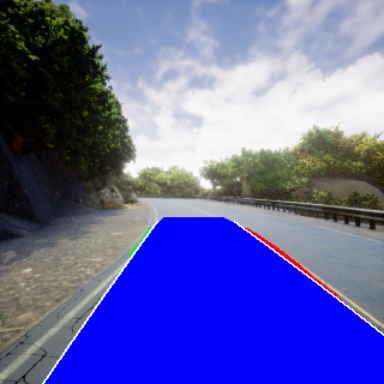
\includegraphics[scale= 0.4]{figs/Diseño/Regresiones/interpolacion.jpg}
    \end{center}
    \caption{Resultado de la interpolación}
    \label{fig:interpolación}
  \end{figure}\

  Finalmente, cuando obtengamos el cálculo del carril que queremos seguir solamente faltará calcular el centro de masas de dicho fragmento conocido como el centroide siguiendo la ecuación
  del cálculo de centro de masas de una superficie. \newline

  \begin{equation} 
    \vec{r}_{CM} = \frac{\sum_{i}m_{i} \vec{r}_{i}}{\sum_{i}m_{i}} = \frac{\sum_{i}m_{i} \vec{r}_{i}}{M} 
    \newline
  \end{equation} 
 
  Para ello, 
  supondremos que todos los puntos tienen la misma masa (m\_i = 1). Esto simplifica el cálculo, pero en aplicaciones del mundo real, las masas pueden variar.
  El segundo paso será el calculo de la masa total, se calcula multiplicando la masa individual (m\_i) por la cantidad de puntos en el carril. A continuación calcularemos
  la suma de las posiciones de los puntos ponderadas por su masa y dividimos por la masa total calculada anteriormente. El resultado es una centro de masas conocido como centroide
  con coordenada x e y. 

  \begin{figure} [H]
    \begin{center}
      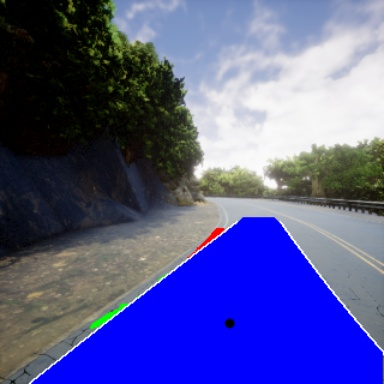
\includegraphics[scale=0.6]{figs/Diseño/Regresiones/percepcion.jpg}
    \end{center}
    \caption{Resultado del centro de masas}
    \label{fig:centro de masas}
  \end{figure}\

  \section{Navegación autonóma mediante un controlador PID}
  \label{sec:Control}

  Una vez realizado el comportamiento de la percepción, construiremos un comportamiento autónomo con el dron basandonos en un simple controlador PID utilizando como controladores de vuelo
  y movimiento con PX4 y Mavros. 
  Como comentamos en la sección \ref{subsec:Configuración del dron y del entorno} configuramos dichos parametros de PX4 para el comportamiento del dron. A continuación comentaremos los parametros
  y para que nos sirve cada uno de ellos:

  \begin{enumerate}
    \item CBRK\_IO\_SAFETY: Es un interruptor de seguridad 
    \item COM\_ARM\_CHK\_ESCS: 
    \item COM\_ARM\_EKF\_HGT: 
    \item COM\_ARM\_EKF\_POS:
    \item COM\_ARM\_EKF\_VEL:
    \item COM\_ARM\_EKF\_YAW:
    \item COM\_FAIL\_ACT\_T:
    \item COM\_FLIGHT\_UUID:
    \item COM\_OBL\_RC\_ACT:
    \item COM\_PREARM\_MODE:
    \item FD\_ACT\_EN:
    \item LPE\_LAT:
    \item LPE\_LON:
    \item MIS\_TAKEOFF\_ALT:
    \item MPC\_TKO\_SPEED:
    \item MPC\_Z\_VEL\_MAX\_DN:
    \item MPC\_Z\_VEL\_MAX\_UP:
    \item MPC\_Z\_V\_AUTO\_DN:
    \item MPC\_Z\_V\_AUTO\_UP:
    \item NAV\_DLL\_ACT:
    \item NAV\_RCL\_ACT:
    \item SIM\_BAT\_DRAIN:
    \item SIM\_BAT\_MIN\_PCT:
    \item SYS\_FAILURE\_EN:
    \item SYS\_HITL:
  \end{enumerate}

  PX4 ofrece bastantes parametros según las necesidades del desarrollador, en nuestro con estos veinticinco parametros nos bastará para realizar el comportamiento autonónomo junto con los
  modos de vuelo mencionados en la sección \ref{sec:flight modes}. \newline

  Con este primer comportamiento queremos demostrar la funcionalidad de la percepción utilizando un controlador de movimiento sencillo. Un controlador PID (proporcional, derivativo e integral) es un 
  es un sistema que es capaz de mantener una variable (como la temperatura, velocidad o posición) cercana a un valor deseado o de referencia. Cada componente de un controlador tiene un papel 
  importante. \break
  La componente P (proporcional) ajusta la salida del controlador en función de la diferencia entre el valor medido y el valor deseado. 
  Cuanto mayor sea esta diferencia (error), mayor será la corrección aplicada. Sin embargo, el control proporcional solo no puede eliminar completamente el error por ello se utiliza
  las componentes derivativa e integral. La componente D (derivativa) considera la tasa de cambio del error. 
  Si el error cambia rápidamente, el término derivativo aplicará una corrección para evitar oscilaciones o inestabilidad. Es especialmente útil para sistemas con inercia o retraso.
  Y con el término integral acumula el error a lo largo del tiempo y ajusta la salida del controlador en función de esta acumulación. 
  Ayuda a eliminar el error persistente o constante. Si el error es pequeño pero persistente, el término integral lo corregirá gradualmente.
  \newline
 

  Lo cual con este controlador PID sencillo controlaremos las velocidades respecto al error que se produce entre posición deseada y la que obtenemos. La variable deseada para estar alineados con el carril escogeremos 
  en el eje de las x el valor central de la imagen, ya que queremos en todo momento permanecer centrales, para calcular el error realizaremos la diferencia del valor deseado que seria 
  el valor central de la imagen y el valor del centroide del carril mencionado en la sección \ref{sec:Interpolación y cálculo del centro de masas del carril}. 
  A parte de este controlador, utilizaremos un pequeño controlador PD para la altitud del vehículo, aunque PX4 tenga sus controladores internos con ellos no es suficiente ya que al tener
  la componente de la altura con el comportamiento de la percepción, unas desviaciones de altura pueden hacer que la percepción la parte de la red neuronal no tenga una buena detencción, 
  por ello con esta solución es factible para controlar las pequeñas desviaciones de altitud que tenga el vehículo. Para saber a que altitud nos encontramos utilizaremos el sensor del Lidar
  que nos proporciona AirSim ROS Wrapper Node ya que Mavros no proporciona ningún topic con este sensor.

  Para encontrar las valores de cada término que compone ambos controladores se ha realizado a base de experimentación, empezando de manera creciente, es decir, primero utilizariamos
  la componente proporcional para ver su comportamiento, una vez que tengamos el valor del término proporcional pasaremos al termino derivativo para suavizar los movimientos que puede
  producir este término y por último utilizariamos la parte integral para eliminar el error. 

  Además el controlador PID mantendrá una velocidad lineal fija determinada con un valor de 1.5 m/s, dicha velocidad lineal es baja ya que si dicha velocidad es alta puede desembocar
  un comportamiento demasiado agresivo para controlar la posición del vehículo con el carril.

  \section{Navegación autonóma mediante Reinforcement learning}
  \label{sec:Reinforcement learning}
  En esta sección se explicará el funcionamiento del control mediante un Reinforcement Learning. \newline
  Como mencionamos en la sección \ref{sec:IA},Reinforcement Learning es una disciplina de Q-Learning que consiste en enseñar un agente 
  desempeñar un comportamiento mediante recompensas y penalizaciones. Este comportamiento se aprende a base de interacciones con el entorno de trabajo y observaciones de como puede responder,
  de forma similar a los niños que exploran el mundo que les rodea y aprenden las acciones que les ayudan a alcanzar un objetivo. Además, reinforcement learning es un algoritmo muy potente, 
  ya que puede aprender las acciones que conducen al éxito en un entorno desconocido sin la ayuda de un supervisor. \newline

  Este algoritmo se compone se varios componentes que hay que conocer para desarrollar el comportamiento: 
  \begin{itemize} 
    \item Agente: El agente es una entidad o modelo que pretendemos entrenar para que aprenda a tomar decisiones (acciones) en función del estado en el que nos encontremos.
    \item Entorno: Ambiente en donde interactua el agente para que pueda aprendar el comportamiento deseado.
    \item Estados: Condiciones en las que se puede encontrar el agente en ese instante de tiempo
    \item Acciones: Movimientos que puede realizar el agente dentro del estado en el entorno de entrenamiento.
    \item Función de Recompensa o Penalizaciones: Consiste en como queremos premiar o penalizar al agente con el objetivo que queremos cumplir. Las recompensas o penalizaciones se recogen
    en una función, dicha función es independiente en cada diseño del objetivo que quiere completar el agente. 
    \item Política: Determina que acción realizar en cada estado que se encuentre el agente. Dicha política varía según el tipo de algoritmo que queremos seguir dentro de Reinforcement learning.
    Puede ser determinista o estocástica. 
  \end{itemize}

  \begin{figure} [H]
    \begin{center}
      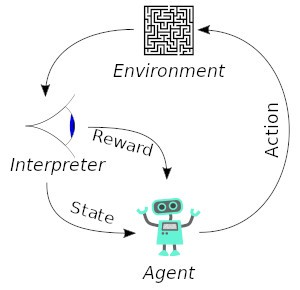
\includegraphics[width=0.5\textwidth,height=0.5\textwidth]{figs/Diseño/RL/Esquema.jpeg}
    \end{center}
    \caption{Esquema de Reinforcement Learning}
    \label{fig:esquemaRL}
  \end{figure}

  Reinforcement learning puede seguir distintos enfoques respecto al algoritmo que tenga como por ejemplo Q-Learning, Deep Q Networks, Policy Gradient Methods, Actor-Critic, 
  Proximal Policy Optimization (PPO) y Métodos de Monte Carlo. Nosotros seguiremos un algoritmo Q-Learning. 
  
  
  \subsection{Sigue carril mediante Q-Learning}
  \label{sec:QLearning}
  \subsubsection{Q-Learning}
  \label{sec:QLearning}
  QLearning es un algoritmo de aprendizaje basado en una función acción-recompensa formada por un tabla estado-acción la cual iremos rellenando siguiendo la siguiente ecuación 
  de Bellman: 

  \begin{equation} 
    Q(s, a) = Q(s, a) + \alpha \cdot [R(s, a) + \gamma \cdot \max Q(s', a') - Q(s, a)]
  \end{equation} 

  en donde, 

  \begin{itemize}
    \item $Q(s, a)$: Valor Q para el estado $s$ y la acción $a$. Se trata de una matriz formada por estado y acción.
    \item $\alpha$: Tasa de aprendizaje entre un valor de 0 a 1. Consiste en el porcentaje que daremos al agente para el proceso de aprendizaje, si dicho valor es alto daremos más peso al valor aprendido 
    \item $R(s, a)$: Recompensa por tomar la acción $a$ en el estado $s$. La función de recompensa es crucial en el proceso de aprendizaje del agente, evalua como es favorable o deseable
    es una acción tomada por el agente en el estado que se encuentre. Proporciona información al agente sobre que acciones maximizan la recompensa total a lo largo del tiempo. Dicha función
    de recompensa es diseñada dependiendo de cual sea el objetivo de tu agente. 
    \item $\gamma$: Factor de descuento entre un valor de 0 a 1. Modela la importancia de las recompensas futuras en relación con las recompensas inmediatas, refleja la importancia del agente
    por las recompensas a largo plazo. Un valor alto sifnigicará que le agente valorará mucho las recompensas futuras, mientras que un valor bajo indica que se enfocará más en las recompensas
    inmediatas
    \item $\max Q(s', a')$: Valor Q máximo en el próximo estado $s'$ para todas las acciones posibles $a'$.
\end{itemize}

\subsubsection{Fases de Q-Learning}
\label{sec:fases_ql}
 El proceso de aprendizaje de Q-Learning se compone en dos fases: Entrenamiento e Inferencia. 
 Antes de comenzar explicando cada parte, definiremos algunos conceptos dentro de estas fases: 
 \begin{itemize}
  \item Episodios: Se define episodio como una secuencia completa de interacciones que se produce entre el agente y el entorno. Cada episodio comienza con un estado inicial y consta de una serie 
  de pasos o acciones tomadas por el agente.
  \item Iteraciones (steps): Son los pasos que puede dar un agente en el entorno dentro de un episodio. Estos pasos pueden incluir observaciones del entorno, decisiones tomadas por el agente
  y las consecuentes recompensas o penalizaciones recibidas.
\end{itemize}

 
 La fase de entrenamiento consiste en el que el agente explore todo lo máximo posible en el entorno respecto a los estados que tiene y las acciones que puede tomar, es decir, al comienzo del entrenamiento se inicializará la tabla Q(S,A) a cero todos sus valores, esta representación
 al comienzo es así ya que el agente desconoce por completo el entorno hasta que poco a poco vaya iterando sobre el en cada estado tomando x accion. \newline
 \newline
 Basicamente, en cada iteración del algoritmo se escogerá una acción según la política que queremos seguir, dicha acción puede ser aleatoria o no, cuando la acción es aleatoria se denomina exploración ya que estamos dejando que el 
 agente inspeccioné las acciones en ese estado concreto y obtenga la mayor recompensa que pueda tener. 
 En cambio si la acción no es aleatoria, se denonima explotación, el objetivo
 principal que tiene la explotación es escoger la acción más conocida que obtenga mayor recompensa en ese estado en el que se encuentre el agente. Cuando se habla de escoger la acción debe 
 haber un equilibrio entre exploración y explotación ya que si la explotación es mayor frente a la exploración puede que el agente no haya inspeccionado todos los estados y acciones 
 posibles y no pueda cumplir el objetivo, también ocurre que si la exploración es mayor que la explotación puede que el agente pierda obtener recompensas altas. \newline
 \newline
 Cuando se escogé la acción ya sea exploración o explotación, dicha acción se ejecuta, se calcula la recompensa obtenida en dicho estado tomando la acción, se obtiene el estado nuevo en el que 
 nos encontramos y calculamos el valor en la tabla Q(S,A), y volvemos a iterar desde el comienzo. \newline
 \newline
 El entrenamiento finaliza cuando el agente haya aprendido el objetivo que queremos seguir, esto se sabe cuando las iteraciones del algoritmo y la recompensa acumulada del agente en esta 
 fase se estabilice y tenga valores constantes, es decir, no cambia significativamente con más iteraciones, esto se denomina que el modelo ha convergido y pasaremos a la fase de inferencia. 


 \begin{figure} [H]
  \begin{center}
    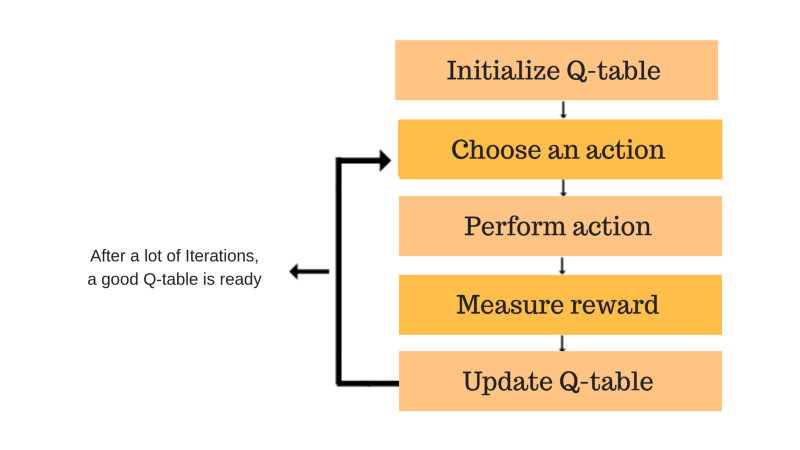
\includegraphics[width=0.8\textwidth,height=0.5\textwidth]{figs/Diseño/RL/entrenamiento.png}
  \end{center}
  \caption{Esquema general del algoritmo de Q-Learning en la fase de entrenamiento}
  \label{fig:algoritmo de Q-Learning}
\end{figure}

La fase de inferencia consiste en indexar la tabla Q(S,A) que hemos ido rellenando en la fase de entrenamiento. El agente cuando se encuentré en un estado especifico consultará la tabla Q(S,A) para
encontrar la mejor acción en ese estado, cuando mencionamos la mejor acción nos referimos al máximo valor en la tabla que tenga en ese estado, el agente toma dicha acción y se mueve al siguiente estado
siendo así un proceso iterativo hasta alcanzar la meta. En esta fase, los valores de la tabla permanecen constantes y se utiliza para la toma de decisiones basadas en el conocimiento
aprendido en la fase de entrenamiento. 

\subsubsection{ Decayed Epsilon-greedy}
\label{sec:epsilon}
Dentro de Q-Learning existen multiples tecnicas a seguir, nosotros seguiremos la política de epsilon-greedy\footnote{\textbf{Epsilon-Greedy}: \url{https://www.baeldung.com/cs/epsilon-greedy-q-learning}}. Epsilon-greedy consiste es una estrategia utilizada dentro del algoritmo
de Q-learning para equilibrar la exploración y explotación en la fase de entrenamiento de Q-Learning. \newline

El agente en la fase de entrenamiento cuando tiene que escoger la acción que tomar como hemos explicado en la sección \ref{sec:fases_ql} puede ser aleatoria o no dependiendo de la política.
Siguiendo esta política, permite al agente tomar decisiones basadas en dos enfoques:

\begin{itemize}
  \item Exploración (con probabilidad $\epsilon$): El agente escogerá una acción al azar para explorar
  \item Explotación(con probabilidad $ 1 - \epsilon$): El agente escogerá la acción con el valor de la tabla Q(S,A) más alto, es decir, la mejor acción conocida
\end{itemize}

El parámetro $\epsilon$ es el responsable de controlar la proporción de exploración frente a explotación, si $\epsilon$  es alto el agente explorará más en cambio si $\epsilon$ es bajo
el agente se centrará en la explotación. Por lo que en la elección de acción se generará un numero n aleatoriamente, si n es menor que la probabilidad $\epsilon$ la acción se escogerá aleatoriamente
en cambio si n es mayor que la probabilidad de $\epsilon$ la acción será que mayor valor tenga en la tabla Q(S,A) para dicho estado. \newline

Dentro de esta política la probabilidad de $\epsilon$ sera decayente, es decir, no ser un valor constante en cada episodio que nos encontremos, lo que realizaremos sera una disminuición 
de esta probabilidad para conseguir que el agente con el paso del tiempo poco a poco explote lo que ha aprendido y que el modelo llegue a una convergencia óptima. Para llevar a cabo el decaimiento
de $\epsilon$ se puede realizar de varias formas, por ejemplo podemos realizarlo linealmente, logaritmicamente, exponencial o escalonado. 

\subsubsection{Definición de variables en el sigue carril mediante Q-Learning}
\label{sec:QLearning}

Una vez definido y explicado detalladamente el algoritmo de Q-learning con la política Decayed Epsilon-greedy, proderemos a definir los componentes
para abordar el problema del sigue carril para un dron

\begin{itemize}
  \item Estados: Para la definición de los estados, dividiremos la imagen que damos como la salida de la detencción del carril en 14 franjas, dichas franjas tendrán una 
  separación de 10 pixeles. Las franjas representarán cada estado en el que se puede encontrar el agente.Empezaremos a definir el primer estado desde la izquierda hasta la derecha
  hasta conseguir los 14 estados correspondientes, 7 estados izquierda, 1 estado central y 6 estados derecha. 
  \item Acciones: Tendremos en total 21 acciones que podrá escoger el agente en el algoritmo de Q-Learning, se componen de pares de velocidades lineales y angulares. Las velocidades lineales
  tendrán un intervalo de 1.45 m/s hasta 2.45 m/s, así siendo el intervalo de la velocidad angular de -0.25 hasta 0.25, teniendo giros hacia la izquierda y hacia la derecha. Dichos pares
  de velocidades serán formados a partir de la función que nos proporciona numpy linspace  
  
\end{itemize}






  


  




  














        


  

